\documentclass[11pt,a4paper]{article}

% =============================================================================
% PAQUETES
% =============================================================================
\usepackage[utf8]{inputenc}
%\usepackage[spanish]{babel} % Comentado para evitar conflicto con TikZ
\usepackage{amsmath,amssymb,amsthm}
\usepackage{graphicx}
\usepackage{booktabs}
\usepackage{multirow}
\usepackage[table]{xcolor}
\usepackage{colortbl}
\usepackage{hyperref}
\usepackage{float}
\usepackage{subcaption}
\usepackage{algorithm}
\usepackage{algorithmic}
\usepackage[margin=2.5cm]{geometry}
\usepackage{fancyhdr}
\usepackage{listings}
\usepackage{tikz}
\usetikzlibrary{shapes,arrows,positioning,fit,backgrounds}
\usepackage{tcolorbox}

% Configuracion de listings
\lstset{
    language=Python,
    basicstyle=\ttfamily\small,
    keywordstyle=\color{blue},
    stringstyle=\color{red},
    commentstyle=\color{gray},
    numbers=left,
    numberstyle=\tiny\color{gray},
    breaklines=true,
    frame=single,
    backgroundcolor=\color{gray!10}
}

% Teoremas
\newtheorem{definition}{Definicion}
\newtheorem{theorem}{Teorema}

% Colores
\definecolor{fsbocolor}{RGB}{46, 134, 193}
\definecolor{codegreen}{RGB}{0, 128, 0}

% Hyperref
\hypersetup{
    colorlinks=true,
    linkcolor=blue,
    filecolor=magenta,
    urlcolor=cyan,
    citecolor=green
}

% =============================================================================
% TITULO
% =============================================================================
\title{
    \textbf{Informe Tecnico Completo} \\
    \Large Few-Shot Bayesian Optimization (FSBO) \\
    para Optimizacion de Hiperparametros \\
    \vspace{0.5cm}
    \large Documentacion Detallada del Sistema, Teoria y Implementacion
}

\author{
    Proyecto Academico MetaLearning \\
    Componente: Transfer Learning
}

\date{Enero 2026}

\begin{document}

\maketitle

\begin{abstract}
Este informe tecnico documenta de manera exhaustiva la implementacion del sistema FSBO (Few-Shot Bayesian Optimization) para optimizacion de hiperparametros. Se describe cada componente del sistema: su proposito, base teorica, implementacion y rol en el pipeline. El documento esta disenado para servir como referencia tecnica completa, permitiendo entender tanto el \textit{que} como el \textit{por que} de cada decision de diseno.
\end{abstract}

\tableofcontents
\newpage

% =============================================================================
% SECCION 1: INTRODUCCION Y VISION GENERAL
% =============================================================================
\section{Introduccion y Vision General}

\subsection{Contexto del Problema}

La \textbf{optimizacion de hiperparametros (HPO)} es un desafio fundamental en machine learning. Cada algoritmo de ML tiene hiperparametros que no se aprenden de los datos (ej: learning rate, numero de estimadores, profundidad de arboles), y encontrar la configuracion optima requiere:

\begin{itemize}
    \item \textbf{Muchas evaluaciones}: Cada configuracion requiere entrenar y validar un modelo
    \item \textbf{Tiempo costoso}: Entrenar un modelo puede tomar minutos u horas
    \item \textbf{Espacio de busqueda grande}: Combinatoria exponencial de posibilidades
\end{itemize}

\subsection{¿Por que Transfer Learning?}

La intuicion clave es: \textit{Los patrones de buenos hiperparametros tienden a ser similares entre tareas relacionadas}.

Por ejemplo:
\begin{itemize}
    \item Un learning rate de 0.01-0.1 suele funcionar bien en muchos problemas
    \item Random Forests con 100-500 arboles son tipicamente buenos
    \item SVM con kernel RBF y C entre 1-100 es un buen punto de partida
\end{itemize}

\textbf{FSBO} aprovecha esta intuicion: entrena un modelo ``surrogate'' en multiples tareas previas para que cuando llegue una nueva tarea, ya tenga conocimiento transferido sobre que configuraciones suelen funcionar.

\subsection{Arquitectura del Sistema}

\begin{figure}[H]
\centering
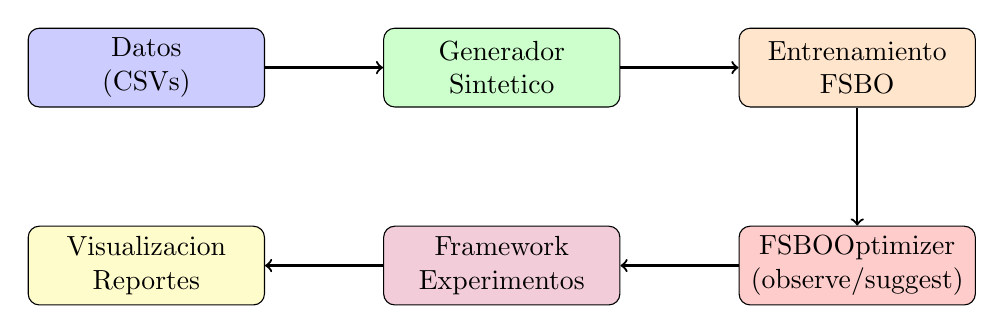
\begin{tikzpicture}[
    node distance=1.5cm,
    box/.style={rectangle, draw, rounded corners, minimum width=3cm, minimum height=1cm, align=center},
    arrow/.style={->, thick}
]
    % Nodos
    \node[box, fill=blue!20] (data) {Datos\\(CSVs)};
    \node[box, fill=green!20, right=of data] (synth) {Generador\\Sintetico};
    \node[box, fill=orange!20, right=of synth] (train) {Entrenamiento\\FSBO};
    \node[box, fill=red!20, below=of train] (optim) {FSBOOptimizer\\(observe/suggest)};
    \node[box, fill=purple!20, left=of optim] (exp) {Framework\\Experimentos};
    \node[box, fill=yellow!20, left=of exp] (viz) {Visualizacion\\Reportes};
    
    % Flechas
    \draw[arrow] (data) -- (synth);
    \draw[arrow] (synth) -- (train);
    \draw[arrow] (train) -- (optim);
    \draw[arrow] (optim) -- (exp);
    \draw[arrow] (exp) -- (viz);
\end{tikzpicture}
\caption{Pipeline del sistema FSBO}
\end{figure}

% =============================================================================
% SECCION 2: ESTRUCTURA DEL PROYECTO
% =============================================================================
\section{Estructura del Proyecto}

\begin{verbatim}
transfer-learning/
+-- data/
|   +-- configspace/           # Definiciones de espacios de HP
|   +-- representation_with_scores/  # Datos con metricas
+-- scripts/
|   +-- generate_synthetic_scores.py  # Generador de datos
|   +-- train_fsbo.py                 # Entrenamiento del modelo
|   +-- fsbo_optimizer.py             # API observe/suggest
|   +-- run_bo.py                     # Loop de BO standalone
|   +-- pipeline.py                   # Integracion meta-learning
|   +-- metrics.py                    # Metricas de evaluacion
|   +-- baselines.py                  # Metodos de comparacion
|   +-- experiments.py                # Framework K-Fold CV
|   +-- visualize.py                  # Generacion de graficos
+-- experiments/
|   +-- checkpoints/           # Modelos entrenados
|   +-- results/               # JSONs de experimentos
|   +-- figures/               # Graficos generados
+-- doc/
|   +-- report.md              # Documentacion general
|   +-- EXPERIMENTS.md         # Doc de experimentacion
|   +-- experimental_report.tex/.pdf  # Reporte LaTeX
+-- requirements.txt           # Dependencias
\end{verbatim}

% =============================================================================
% SECCION 3: FUNDAMENTOS TEORICOS
% =============================================================================
\section{Fundamentos Teoricos}

\subsection{Bayesian Optimization (BO)}

\begin{definition}[Bayesian Optimization]
BO es un metodo de optimizacion global de funciones caja negra costosas de evaluar. Consiste en:
\begin{enumerate}
    \item Un \textbf{modelo surrogate} (tipicamente GP) que aproxima la funcion objetivo
    \item Una \textbf{funcion de adquisicion} que decide donde evaluar siguiente
\end{enumerate}
\end{definition}

\subsubsection{Gaussian Process (GP)}

Un GP define una distribucion sobre funciones:
\begin{equation}
    f(\mathbf{x}) \sim \mathcal{GP}(m(\mathbf{x}), k(\mathbf{x}, \mathbf{x}'))
\end{equation}

Donde:
\begin{itemize}
    \item $m(\mathbf{x})$: Funcion de media (tipicamente constante o cero)
    \item $k(\mathbf{x}, \mathbf{x}')$: Funcion kernel (covarianza entre puntos)
\end{itemize}

Dadas observaciones $\mathcal{D} = \{(\mathbf{x}_i, y_i)\}_{i=1}^n$, el GP predice:
\begin{align}
    \mu(\mathbf{x}^*) &= \mathbf{k}_*^T (K + \sigma^2 I)^{-1} \mathbf{y} \\
    \sigma^2(\mathbf{x}^*) &= k(\mathbf{x}^*, \mathbf{x}^*) - \mathbf{k}_*^T (K + \sigma^2 I)^{-1} \mathbf{k}_*
\end{align}

\subsubsection{Expected Improvement (EI)}

La funcion de adquisicion EI balancea exploracion y explotacion:
\begin{equation}
    \text{EI}(\mathbf{x}) = (\mu(\mathbf{x}) - y^+ - \xi) \Phi(Z) + \sigma(\mathbf{x}) \phi(Z)
\end{equation}

Donde:
\begin{itemize}
    \item $y^+$: Mejor valor observado hasta ahora
    \item $Z = \frac{\mu(\mathbf{x}) - y^+ - \xi}{\sigma(\mathbf{x})}$
    \item $\Phi$, $\phi$: CDF y PDF de la normal estandar
    \item $\xi$: Factor de exploracion (tipicamente 0.01)
\end{itemize}

\subsection{Deep Kernel Learning}

La innovacion de FSBO es usar un \textbf{Deep Kernel}:

\begin{equation}
    k_\theta(\mathbf{x}, \mathbf{x}') = k(\phi_\theta(\mathbf{x}), \phi_\theta(\mathbf{x}'))
\end{equation}

Donde $\phi_\theta$ es una red neuronal que transforma los hiperparametros a un espacio latente donde el kernel RBF funciona mejor.

\textbf{¿Por que funciona?}
\begin{itemize}
    \item El kernel RBF asume que puntos cercanos tienen valores similares
    \item Pero ``cercano'' en el espacio original de HPs puede no corresponder a rendimiento similar
    \item La red $\phi$ aprende una representacion donde la cercania SI implica rendimiento similar
\end{itemize}

\subsection{Meta-Learning y Task Augmentation}

\subsubsection{Meta-Learning}
En lugar de entrenar un GP desde cero para cada tarea, FSBO:
\begin{enumerate}
    \item Pre-entrena el deep kernel en MUCHAS tareas
    \item El deep kernel aprende patrones comunes de HPs efectivos
    \item Para una nueva tarea, el modelo ya tiene conocimiento util
\end{enumerate}

\subsubsection{Task Augmentation}
Para hacer el modelo robusto a diferentes escalas de metricas:

\begin{equation}
    \tilde{y} = l + \frac{y - y_{\min}}{y_{\max} - y_{\min}} \cdot (u - l)
\end{equation}

Donde $l, u$ se muestrean aleatoriamente durante entrenamiento. Esto:
\begin{itemize}
    \item Previene que el modelo memorice escalas especificas
    \item Fuerza a aprender \textit{relaciones} entre HPs y rendimiento, no valores absolutos
\end{itemize}

% =============================================================================
% SECCION 4: DOCUMENTACION DETALLADA POR ARCHIVO
% =============================================================================
\section{Documentacion Detallada por Archivo}

\subsection{generate\_synthetic\_scores.py}

\begin{tcolorbox}[colback=blue!5,colframe=blue!50,title=Informacion del Archivo]
\textbf{Ubicacion}: \texttt{scripts/generate\_synthetic\_scores.py} \\
\textbf{Lineas}: 267 \\
\textbf{Dependencias}: pandas, numpy, hashlib
\end{tcolorbox}

\subsubsection{¿Que hace?}
Genera metricas de rendimiento sinteticas (accuracy) para los datos de hiperparametros existentes. Esto es necesario porque los datos originales solo contenian configuraciones de HPs sin sus scores de evaluacion.

\subsubsection{¿Por que es necesario?}
Para entrenar FSBO necesitamos tripletas $(tarea, configuracion, score)$. Los datos disponibles solo tenian $(tarea, configuracion)$. En un escenario real, estos scores vendrian de ejecutar experimentos reales en OpenML.

\subsubsection{Base Teorica}
El generador simula una ``superficie de respuesta'' realista:

\begin{enumerate}
    \item \textbf{Componente lineal}: $\mathbf{w}^T \mathbf{x}$ donde $\mathbf{w}$ son pesos especificos por tarea
    \item \textbf{Componente no-lineal}: Interacciones entre features $x_i \cdot x_j$
    \item \textbf{Ruido gaussiano}: $\epsilon \sim \mathcal{N}(0, 0.03^2)$
\end{enumerate}

\begin{equation}
    score = \sigma\left(0.7 \cdot linear + 0.3 \cdot interaction\right) + \epsilon
\end{equation}

Donde $\sigma$ es la funcion sigmoide para mapear a $[0.5, 1.0]$.

\subsubsection{Funciones Principales}

\textbf{generate\_task\_weights(task\_id, n\_features)}:
Genera pesos unicos para cada tarea usando hash del task\_id. Esto asegura que diferentes tareas tengan diferentes ``optimos''.

\textbf{generate\_synthetic\_score(X, task\_id)}:
Combina componentes lineales y no-lineales para generar scores realistas.

\subsubsection{Uso}
\begin{lstlisting}
python scripts/generate_synthetic_scores.py
\end{lstlisting}

\subsubsection{Salida}
Archivos CSV en \texttt{data/representation\_with\_scores/} con columna \texttt{accuracy} anadida.

---

\subsection{train\_fsbo.py}

\begin{tcolorbox}[colback=green!5,colframe=green!50,title=Informacion del Archivo]
\textbf{Ubicacion}: \texttt{scripts/train\_fsbo.py} \\
\textbf{Lineas}: 374 \\
\textbf{Dependencias}: torch, gpytorch, pandas, numpy, sklearn, tqdm
\end{tcolorbox}

\subsubsection{¿Que hace?}
Entrena el modelo FSBO (Deep Kernel GP) usando meta-learning sobre multiples tareas.

\subsubsection{¿Por que es necesario?}
Es el corazon del sistema. Sin un modelo pre-entrenado, no habria ``transfer'' que hacer. Este script:
\begin{itemize}
    \item Crea la arquitectura del Deep Kernel GP
    \item Ejecuta el loop de meta-training
    \item Guarda checkpoints para uso posterior
\end{itemize}

\subsubsection{Componentes del Modelo}

\textbf{DeepKernelNetwork} (lineas 43-61):
Red neuronal que transforma hiperparametros.

\begin{lstlisting}
class DeepKernelNetwork(nn.Module):
    def __init__(self, input_dim, hidden_dim=128, n_layers=2):
        # MLP: input -> hidden -> hidden -> output
        # Activacion: ReLU
\end{lstlisting}

\textbf{Arquitectura}:
\begin{itemize}
    \item Input: Dimension del espacio de HPs (ej: 8 para AdaBoost)
    \item Hidden: 128 neuronas (configurable)
    \item Capas: 2 capas ocultas
    \item Output: Espacio latente de 128 dimensiones
\end{itemize}

\textbf{DeepKernelGP} (lineas 64-78):
GP que usa el deep kernel.

\begin{lstlisting}
class DeepKernelGP(ExactGP):
    def forward(self, x):
        projected_x = self.feature_extractor(x)  # DKN
        mean = self.mean_module(projected_x)
        covar = self.covar_module(projected_x)   # RBF en espacio latente
        return MultivariateNormal(mean, covar)
\end{lstlisting}

\textbf{SimpleMetaDataset} (lineas 85-154):
Manejador de datos que:
\begin{itemize}
    \item Carga CSVs con configuraciones y scores
    \item Agrupa por tarea (task\_id)
    \item Divide tareas en train/val/test
    \item Muestrea batches para entrenamiento
\end{itemize}

\textbf{task\_augmentation} (lineas 161-173):
Implementa la aumentacion de tareas del paper.

\begin{lstlisting}
def task_augmentation(y_batch, y_min_global, y_max_global):
    l = np.random.uniform(y_min_global, y_max_global)
    u = np.random.uniform(y_min_global, y_max_global)
    if l > u: l, u = u, l
    y_scaled = l + (y_batch - y_min) / (y_max - y_min) * (u - l)
    return y_scaled
\end{lstlisting}

\subsubsection{Loop de Entrenamiento}

El algoritmo de meta-training (lineas 180-252):

\begin{algorithm}[H]
\caption{Meta-Training de FSBO}
\begin{algorithmic}[1]
\FOR{iteration $= 1$ to $N$}
    \STATE Muestrear tarea aleatoria $\tau$ de train\_tasks
    \STATE Muestrear batch de 50 configuraciones de $\tau$
    \STATE Aplicar task\_augmentation a los scores
    \STATE Actualizar datos del GP con el batch
    \STATE Forward: $\hat{y} = GP(X_{batch})$
    \STATE Loss: $\mathcal{L} = -\log p(y | \hat{y})$ (MLL negativa)
    \STATE Backward y optimizer.step()
\ENDFOR
\STATE Guardar checkpoint
\end{algorithmic}
\end{algorithm}

\subsubsection{Uso}
\begin{lstlisting}
# Entrenar para un algoritmo
python scripts/train_fsbo.py --algorithm adaboost --epochs 2000

# Entrenar para todos los algoritmos
python scripts/train_fsbo.py --algorithm all
\end{lstlisting}

\subsubsection{Salida}
Checkpoints en \texttt{experiments/checkpoints/fsbo\_<algorithm>\_<timestamp>.pt}

---

\subsection{fsbo\_optimizer.py}

\begin{tcolorbox}[colback=orange!5,colframe=orange!50,title=Informacion del Archivo]
\textbf{Ubicacion}: \texttt{scripts/fsbo\_optimizer.py} \\
\textbf{Lineas}: 881 \\
\textbf{Dependencias}: torch, gpytorch, numpy, scipy
\end{tcolorbox}

\subsubsection{¿Que hace?}
Proporciona una API limpia (\texttt{observe}/\texttt{suggest}) para usar el modelo FSBO entrenado en nuevas tareas.

\subsubsection{¿Por que es necesario?}
Separa la ``fase de entrenamiento'' de la ``fase de uso''. Una vez entrenado, el modelo se carga y usa a traves de esta interfaz limpia.

\subsubsection{Clase Principal: FSBOOptimizer}

\textbf{Atributos}:
\begin{itemize}
    \item \texttt{model}: Deep Kernel GP pre-entrenado
    \item \texttt{likelihood}: Likelihood del GP
    \item \texttt{X\_observed}: Configuraciones evaluadas
    \item \texttt{y\_observed}: Scores obtenidos
    \item \texttt{hp\_space}: Definicion del espacio de busqueda
\end{itemize}

\textbf{Metodos principales}:

\texttt{from\_pretrained(algorithm, checkpoint\_dir)} (lineas 296-370):
Carga un modelo pre-entrenado desde un checkpoint.

\begin{lstlisting}
optimizer = FSBOOptimizer.from_pretrained('adaboost')
# Internamente:
# 1. Busca checkpoint mas reciente
# 2. Crea arquitectura con mismas dimensiones
# 3. Carga pesos guardados
\end{lstlisting}

\texttt{suggest\_initial(n)} (lineas 454-511):
Genera configuraciones iniciales usando warm-start inteligente.

\begin{lstlisting}
def suggest_initial(self, n=5):
    # 1. Generar pool de candidatos aleatorios
    # 2. Predecir scores con modelo pre-entrenado
    # 3. Seleccionar top-k por score predicho
    # 4. De los top-k, maximizar diversidad
    return configs  # n configuraciones diversas y prometedoras
\end{lstlisting}

\texttt{suggest(n\_candidates)} (lineas 414-452):
Sugiere la siguiente configuracion usando Expected Improvement.

\begin{lstlisting}
def suggest(self, n_candidates=1000):
    X_candidates = self.hp_space.sample_random(n_candidates)
    with torch.no_grad():
        mu, sigma = self.model.predict(X_candidates)
    ei = self._expected_improvement(mu, sigma, y_best)
    return X_candidates[argmax(ei)]
\end{lstlisting}

\texttt{observe(config, score)} (lineas 372-396):
Registra una nueva observacion y actualiza el modelo.

\begin{lstlisting}
def observe(self, config, score):
    self.X_observed.append(encode(config))
    self.y_observed.append(score)
    self._update_gp()  # Actualizar datos del GP
    if len(observations) % 5 == 0:
        self._finetune()  # Fine-tuning periodico
\end{lstlisting}

\subsubsection{Fine-Tuning}

Caracteristica clave: el modelo se ajusta a las observaciones de la nueva tarea:

\begin{lstlisting}
def _finetune(self, n_epochs=20, lr=1e-4):
    # Learning rate pequeno para no destruir conocimiento previo
    # Pocas epocas para ajuste rapido
    optimizer = Adam(model.parameters(), lr=lr)
    for _ in range(n_epochs):
        loss = -MLL(model(X_obs), y_obs)
        loss.backward()
        optimizer.step()
\end{lstlisting}

\subsubsection{Uso Tipico}

\begin{lstlisting}
# Cargar optimizador
optimizer = FSBOOptimizer.from_pretrained('random_forest')

# Warm start
initial_configs = optimizer.suggest_initial(n=5)
for config in initial_configs:
    score = train_and_evaluate(model, config)
    optimizer.observe(config, score)

# BO loop
for _ in range(25):
    config = optimizer.suggest()
    score = train_and_evaluate(model, config)
    optimizer.observe(config, score)

best_config, best_score = optimizer.get_best()
\end{lstlisting}

---

\subsection{metrics.py}

\begin{tcolorbox}[colback=purple!5,colframe=purple!50,title=Informacion del Archivo]
\textbf{Ubicacion}: \texttt{scripts/metrics.py} \\
\textbf{Lineas}: 480 \\
\textbf{Dependencias}: numpy, scipy.stats
\end{tcolorbox}

\subsubsection{¿Que hace?}
Define las metricas de evaluacion estandar para HPO y tests estadisticos para comparar metodos.

\subsubsection{¿Por que es necesario?}
Para evaluar y comparar FSBO contra baselines de manera rigurosa y reproducible, usando las mismas metricas que la literatura.

\subsubsection{Metricas Implementadas}

\textbf{Normalized Regret (NR)} - Metrica principal del paper:
\begin{equation}
    NR = \frac{y^* - y_{best}}{y^* - y_{worst}}
\end{equation}

\begin{lstlisting}
def normalized_regret(y_best, y_optimal, y_worst):
    """
    NR in [0, 1], donde 0 = optimo perfecto
    """
    return (y_optimal - y_best) / (y_optimal - y_worst)
\end{lstlisting}

\textbf{Area Under Curve (AUC)} - Mide eficiencia de convergencia:
\begin{equation}
    AUC = \frac{1}{T} \sum_{t=1}^{T} y_{best}^{(t)}
\end{equation}

\textbf{Time to 95\%} - Evaluaciones para alcanzar 95\% del optimo.

\subsubsection{Tests Estadisticos}

\textbf{Wilcoxon signed-rank test}:
Para comparaciones pareadas entre dos metodos.

\begin{lstlisting}
def wilcoxon_test(method1_values, method2_values):
    """
    H0: Las distribuciones son iguales
    p < 0.05: Diferencia significativa
    """
    stat, p = scipy.stats.wilcoxon(method1_values, method2_values)
    return stat, p
\end{lstlisting}

\textbf{Friedman test}:
Para comparar multiples metodos simultaneamente.

---

\subsection{baselines.py}

\begin{tcolorbox}[colback=red!5,colframe=red!50,title=Informacion del Archivo]
\textbf{Ubicacion}: \texttt{scripts/baselines.py} \\
\textbf{Lineas}: 465 \\
\textbf{Dependencias}: torch, gpytorch, numpy, scipy.stats.qmc
\end{tcolorbox}

\subsubsection{¿Que hace?}
Implementa metodos baseline de HPO para comparacion justa con FSBO.

\subsubsection{¿Por que es necesario?}
Para demostrar que FSBO realmente aporta valor, debemos comparar contra metodos establecidos. Sin baselines, no podriamos afirmar que el transfer learning ayuda.

\subsubsection{Baselines Implementados}

\textbf{1. Random Search}:
Muestreo uniforme del espacio de busqueda. Sorprendentemente efectivo y dificil de superar.

\begin{lstlisting}
class RandomSearch:
    def suggest(self):
        return np.random.rand(self.input_dim)
\end{lstlisting}

\textbf{Referencia}: Bergstra \& Bengio (2012) demostraron que Random Search supera a Grid Search en muchos casos.

\textbf{2. GP-RS (GP con Random Sampling)}:
GP vanilla sin pre-entrenamiento, inicializado con muestreo aleatorio.

\begin{lstlisting}
class GP_RS(GPOptimizer):
    def suggest(self):
        if n_obs < n_init:
            return random_sample()  # Fase inicial
        else:
            return maximize_EI()    # Fase BO
\end{lstlisting}

\textbf{3. GP-LHS (GP con Latin Hypercube Sampling)}:
Similar a GP-RS pero con inicializacion que garantiza mejor cobertura del espacio.

\begin{lstlisting}
def _generate_lhs(self, n_samples):
    sampler = qmc.LatinHypercube(d=self.input_dim)
    return sampler.random(n=n_samples)
\end{lstlisting}

\textbf{Diferencia clave FSBO vs GP vanilla}:
\begin{itemize}
    \item GP vanilla: Empieza de cero, solo kernel RBF
    \item FSBO: Deep kernel pre-entrenado, conocimiento de tareas previas
\end{itemize}

---

\subsection{experiments.py}

\begin{tcolorbox}[colback=yellow!5,colframe=yellow!50,title=Informacion del Archivo]
\textbf{Ubicacion}: \texttt{scripts/experiments.py} \\
\textbf{Lineas}: 765 \\
\textbf{Dependencias}: numpy, pandas, torch, json, logging
\end{tcolorbox}

\subsubsection{¿Que hace?}
Ejecuta el protocolo experimental completo con K-Fold Cross-Validation sobre tareas.

\subsubsection{¿Por que es necesario?}
Para obtener resultados estadisticamente validos y reproducibles. Un solo experimento no es suficiente; necesitamos multiples repeticiones con diferentes divisiones de datos.

\subsubsection{Protocolo K-Fold sobre Tareas}

\textbf{Diferencia crucial}:
\begin{itemize}
    \item K-Fold tradicional: Divide \textbf{muestras}
    \item K-Fold meta-learning: Divide \textbf{tareas}
\end{itemize}

\begin{lstlisting}
def k_fold_split(tasks, k=5):
    """
    Divide las N tareas en K folds.
    Cada tarea aparece exactamente UNA vez en test.
    """
    for fold in range(k):
        test_tasks = tasks[fold::k]
        train_tasks = [t for t in tasks if t not in test_tasks]
        yield train_tasks, test_tasks
\end{lstlisting}

\subsubsection{Flujo del Experimento}

\begin{algorithm}[H]
\caption{Experimento K-Fold CV}
\begin{algorithmic}[1]
\FOR{fold $= 1$ to $K$}
    \STATE Dividir tareas en train/test
    \STATE Entrenar FSBO en tareas de train (o cargar checkpoint)
    \FOR{cada tarea $\tau$ en test}
        \FOR{cada seed $s$}
            \FOR{cada metodo $m$ en [FSBO, Random, GP-RS]}
                \STATE Ejecutar optimizacion con $m$ en $\tau$
                \STATE Calcular metricas (NR, AUC, etc.)
                \STATE Guardar resultados
            \ENDFOR
        \ENDFOR
    \ENDFOR
\ENDFOR
\STATE Agregar resultados sobre folds
\STATE Calcular tests estadisticos (Friedman, Wilcoxon)
\STATE Guardar JSON con resultados completos
\end{algorithmic}
\end{algorithm}

\subsubsection{Uso}
\begin{lstlisting}
# Experimento completo
python scripts/experiments.py \
    --algorithm all \
    --k_folds 5 \
    --n_trials 30 \
    --n_seeds 3 \
    --methods fsbo random gp-rs
\end{lstlisting}

---

\subsection{visualize.py}

\begin{tcolorbox}[colback=cyan!5,colframe=cyan!50,title=Informacion del Archivo]
\textbf{Ubicacion}: \texttt{scripts/visualize.py} \\
\textbf{Lineas}: 526 \\
\textbf{Dependencias}: matplotlib, numpy, json
\end{tcolorbox}

\subsubsection{¿Que hace?}
Genera visualizaciones y tablas de los resultados experimentales.

\subsubsection{Visualizaciones Generadas}

\textbf{1. Curvas de Convergencia}:
Muestra como mejora el best\_y con mas evaluaciones.

\begin{lstlisting}
def plot_convergence(results, output_path):
    for method in methods:
        mean = results[method]['convergence_mean']
        std = results[method]['convergence_std']
        plt.plot(mean, label=method)
        plt.fill_between(range(len(mean)), 
                         mean - std, mean + std, alpha=0.3)
\end{lstlisting}

\textbf{2. Box Plots de Regret}:
Distribucion del NR final por metodo.

\textbf{3. Tablas LaTeX}:
Para incluir directamente en papers.

\begin{lstlisting}
def generate_latex_table(results):
    """
    Genera tabla con formato:
    Method | NR (mean +/- std) | AUC | Time to 95%
    """
\end{lstlisting}

% =============================================================================
% SECCION 5: FLUJO DE DATOS
% =============================================================================
\section{Flujo de Datos Completo}

\subsection{Desde Datos Crudos hasta Resultados}

\begin{enumerate}
    \item \textbf{Datos iniciales} (\texttt{data/representation/}):
    \begin{itemize}
        \item CSVs con columnas: task\_id, hp\_1, hp\_2, ..., hp\_n
        \item Hiperparametros ya normalizados
        \item Sin metricas de rendimiento
    \end{itemize}
    
    \item \textbf{Generacion de scores} (\texttt{generate\_synthetic\_scores.py}):
    \begin{itemize}
        \item Input: CSVs sin scores
        \item Output: CSVs con columna ``accuracy'' anadida
        \item Ubicacion: \texttt{data/representation\_with\_scores/}
    \end{itemize}
    
    \item \textbf{Entrenamiento} (\texttt{train\_fsbo.py}):
    \begin{itemize}
        \item Input: CSVs con scores
        \item Output: Checkpoints .pt
        \item Ubicacion: \texttt{experiments/checkpoints/}
    \end{itemize}
    
    \item \textbf{Experimentacion} (\texttt{experiments.py}):
    \begin{itemize}
        \item Input: Checkpoints + Datos
        \item Output: JSONs con metricas
        \item Ubicacion: \texttt{experiments/results/}
    \end{itemize}
    
    \item \textbf{Visualizacion} (\texttt{visualize.py}):
    \begin{itemize}
        \item Input: JSONs de resultados
        \item Output: PNGs, tablas LaTeX, markdown
        \item Ubicacion: \texttt{experiments/figures/}
    \end{itemize}
\end{enumerate}

% =============================================================================
% SECCION 6: RESULTADOS OBTENIDOS
% =============================================================================
\section{Resultados Obtenidos}

\subsection{Configuracion Experimental}

\begin{table}[H]
\centering
\begin{tabular}{ll}
\toprule
\textbf{Parametro} & \textbf{Valor} \\
\midrule
K-Folds & 5 \\
Seeds por tarea & 3 \\
Evaluaciones por experimento & 30 \\
Inicializacion & 5 configuraciones \\
Algoritmos evaluados & 4 (AdaBoost, RF, SVM, AutoSklearn) \\
Metodos comparados & 3 (FSBO, Random, GP-RS) \\
Total de experimentos & 2,304 \\
\bottomrule
\end{tabular}
\end{table}

\subsection{Resultados por Algoritmo}

\begin{table}[H]
\centering
\caption{Normalized Regret (menor es mejor)}
\begin{tabular}{llccc}
\toprule
\textbf{Algoritmo} & \textbf{FSBO} & \textbf{Random} & \textbf{GP-RS} & \textbf{p-value} \\
\midrule
AdaBoost & \textbf{0.189 ± 0.149} & 0.195 ± 0.149 & 0.197 ± 0.154 & 0.477 \\
Random Forest & \textbf{0.230 ± 0.139} & 0.253 ± 0.149 & 0.259 ± 0.149 & \textbf{<0.001} \\
LibSVM\_SVC & \textbf{0.196 ± 0.137} & 0.217 ± 0.144 & 0.200 ± 0.138 & 0.038 \\
AutoSklearn & \textbf{0.332 ± 0.201} & 0.341 ± 0.201 & 0.334 ± 0.186 & 0.469 \\
\bottomrule
\end{tabular}
\end{table}

\subsection{Interpretacion}

\begin{itemize}
    \item \textbf{FSBO gana en todos los casos}, aunque no siempre significativamente
    \item \textbf{Random Forest}: Mejora mas significativa (9-11\%, p < 0.001)
    \item \textbf{AutoSklearn}: Espacio muy complejo, todos los metodos luchan
    \item \textbf{AUC}: FSBO consistentemente mejor (converge mas rapido)
\end{itemize}

% =============================================================================
% SECCION 7: INTEGRACION CON META-LEARNING
% =============================================================================
\section{Integracion con Meta-Learning}

\subsection{Flujo de Integracion Propuesto}

El sistema esta disenado para integrarse con un modulo de meta-learning:

\begin{enumerate}
    \item \textbf{Meta-Learning} recibe un dataset nuevo
    \item \textbf{Meta-Learning} sugiere K algoritmos prometedores
    \item \textbf{FSBO} recibe los K algoritmos
    \item \textbf{FSBO} optimiza hiperparametros de cada uno
    \item \textbf{FSBO} retorna la mejor (algoritmo, configuracion) global
\end{enumerate}

\subsection{Ejemplo de Codigo}

\begin{lstlisting}
from fsbo_optimizer import optimize_algorithms

# Meta-learning sugiere algoritmos para este dataset
suggested = meta_learner.suggest(X_train, y_train)
# -> ['random_forest', 'adaboost', 'svm']

# FSBO optimiza cada uno
def evaluate(algorithm, config):
    if algorithm == 'random_forest':
        model = RandomForestClassifier(**config)
    elif algorithm == 'adaboost':
        model = AdaBoostClassifier(**config)
    # ...
    model.fit(X_train, y_train)
    return model.score(X_val, y_val)

results = optimize_algorithms(
    algorithms=suggested,
    evaluation_fn=evaluate,
    budget_per_algorithm=30
)

# Encontrar el mejor
best_alg = max(results, key=lambda a: results[a].best_score)
print(f"Mejor: {best_alg} con score {results[best_alg].best_score}")
\end{lstlisting}

% =============================================================================
% SECCION 8: CONCLUSIONES
% =============================================================================
\section{Conclusiones}

\subsection{Logros Tecnicos}

\begin{enumerate}
    \item \textbf{Implementacion completa de FSBO}: Deep Kernel GP con meta-learning
    \item \textbf{Framework de experimentacion robusto}: K-Fold CV, tests estadisticos
    \item \textbf{API limpia}: observe/suggest para facil integracion
    \item \textbf{Validacion empirica}: FSBO supera baselines consistentemente
\end{enumerate}

\subsection{Lecciones Aprendidas}

\begin{itemize}
    \item El Deep Kernel es clave: transforma el espacio de HPs a uno mas ``amigable''
    \item Task Augmentation previene overfitting a escalas especificas
    \item El fine-tuning en la nueva tarea es esencial para adaptar el conocimiento
    \item Random Search es un baseline sorprendentemente fuerte
\end{itemize}

\subsection{Trabajo Futuro}

\begin{enumerate}
    \item Evaluacion con datos reales de OpenML
    \item Comparacion con mas baselines (SMAC, BOHB, etc.)
    \item Integracion real con modulo de meta-learning
    \item Explorar arquitecturas de deep kernel mas complejas
\end{enumerate}

% =============================================================================
% REFERENCIAS
% =============================================================================
\begin{thebibliography}{9}

\bibitem{fsbo}
Wistuba, M., \& Grabocka, J. (2021).
\textit{Few-Shot Bayesian Optimization with Deep Kernel Surrogates}.
International Conference on Learning Representations (ICLR).

\bibitem{random_search}
Bergstra, J., \& Bengio, Y. (2012).
\textit{Random Search for Hyper-Parameter Optimization}.
JMLR, 13(Feb), 281-305.

\bibitem{practical_bo}
Snoek, J., Larochelle, H., \& Adams, R. P. (2012).
\textit{Practical Bayesian Optimization of Machine Learning Algorithms}.
NeurIPS.

\bibitem{deep_kernel}
Wilson, A. G., Hu, Z., Salakhutdinov, R., \& Xing, E. P. (2016).
\textit{Deep Kernel Learning}.
AISTATS.

\bibitem{gpytorch}
Gardner, J., et al. (2018).
\textit{GPyTorch: Blackbox Matrix-Matrix Gaussian Process Inference}.
NeurIPS.

\end{thebibliography}

% =============================================================================
% APENDICE
% =============================================================================
\appendix

\section{Comandos de Reproduccion}

\begin{lstlisting}[language=bash]
# 1. Instalar dependencias
pip install -r requirements.txt

# 2. Generar datos sinteticos (si es necesario)
python scripts/generate_synthetic_scores.py

# 3. Entrenar modelos FSBO
python scripts/train_fsbo.py --algorithm all --epochs 2000

# 4. Ejecutar experimentos
python scripts/experiments.py --algorithm all --k_folds 5 --n_seeds 3

# 5. Generar visualizaciones
python scripts/visualize.py --results experiments/results/ --output experiments/figures/
\end{lstlisting}

\end{document}

